\documentclass[10pt,a4paper]{scrartcl}
\usepackage[utf8]{inputenc}
\usepackage[francais]{babel}
\usepackage{lmodern}
\usepackage[T1]{fontenc}
\usepackage{xcolor}
\usepackage{graphicx}
\usepackage{amsmath, amssymb, amsthm}
\usepackage{geometry}
\usepackage{thmbox}
\usepackage{enumerate}
\usepackage{subcaption}

\geometry{
a4paper,
body={150mm,260mm},
left=30mm,top=15mm,
headheight=7mm,headsep=4mm,
marginparsep=4mm,
marginparwidth=27mm}


\pagestyle{empty}

\providecommand{\abs}[1]{\left|#1\right|}
\providecommand{\C}{\mathbb{C}}
\providecommand{\R}{\mathbb{R}}
\providecommand{\E}{\mathbb{E}}
\providecommand{\Prob}{\mathbb{P}}
\providecommand{\ii}{\mathrm{i}}
\providecommand{\w}{\omega}
\providecommand{\one}{\textbf{1}}

\renewcommand{\S}{\textbf{S}^n}

\newcommand{\norm}[1]{\Arrowvert#1\Arrowvert_2}

\newcount\colveccount

\newcommand*\colvec[1]{
        \global\colveccount#1
        \begin{pmatrix}
        \colvecnext
}
\def\colvecnext#1{
        #1
        \global\advance\colveccount-1
        \ifnum\colveccount>0
                \\
                \expandafter\colvecnext
        \else
                \end{pmatrix}
        \fi
}
 
\author{Judith Abecassis \& Timothée Lacroix}

\title{Random Graph Bandits with side information}


\begin{document}
\maketitle

\section{Introduction}
\subsection{Context}
We are interesting in a bandit with side informations setting. This consists in a sequential learning where, at each iteration, the learner chooses an arm, and observes losses of a number of arms. This is a generalization of two well-studied feedback settings, one in which the learner only knows the loss of the arm it pulled (bandit setting), and the other where the losses of all arms are revealed (full information setting). Full information occurs for example for trading on a stock market: all stock prices are known, and the bandit setting can be illustrated by electronic advertising. A situation of partial revelation of other arms could be considered in advertising in a social network.

We are following the formalism previouly proposed by Mannor and Shamir (2011) in which side observations are modelled using a graph structure: each possible action is a node, and when an action is chosen, its loss and the losses of all its neighbours in the graph are revealed. Our work is in the line of Valko et al. (2015, under review), and considers the case where no information on the structure of the graph is known, and where partial observation is stochastic. 

We are considering two models of random graphs.

\subsection{Different Graphs models}

\subsubsection{Erdos-Renyi}
Let $0\leq p \leq 1$. $E=ER(p)$ is the graph such that $(i \rightarrow j) \in E$ with probability $p$. Such graphs have very well understood properties. Their expected independence number $\bar{\alpha}$ is ????????.
Examples of ER graphs are given in Fig~\ref{er_ex}.

\begin{figure}
 %\includegraphics{figures/er_graph_1.eps}
 ~
 %\includegraphics{figures/er_graph_2.eps}
 \label{er_ex}
 \caption{Examples of Erdos-Renyi graphs for various $p$}
\end{figure}

In our learning setting, this corresponds to the fact that when an action is chosen, other actions reveal their losses with a constant probability $p$.

\subsubsection{Barabási-Albert}
A Barabási-Albert (BA) graph is constructed dynamically by linking a new node to pre-existing nodes, with a probability linear in the degree of these nodes. As such, a BA graph is parametric, with parameters $m$ and $m0$, namely the number of links a node creates when joining the network, and the size of the starting graph.

These graphs are scale-free, meaning that as they grow, their degree distribution follows a power law :
$$P(k) \equiv k^{-3}~\text{as}~N\rightarrow \infty$$

We used $m=m0=1$ to generate our graphs, leading to the exemples of graphs in figure~\ref{ba_ex}.

\begin{figure}
 %\includegraphics{figures/ba_graph_1.eps}
 ~
 %\includegraphics{figures/ba_graph_2.eps}
 \label{ba_ex}
 \caption{Examples of Barabási-Albert graphs.}
\end{figure}

In our learning setting, this models the phenomenon of preferential attachment in social networks.

\section{ER graphs}
\subsection{Idea of \textsc{DuplExp3} algorithm}
Valko et al. ahev developped an algorithm to learn in the bandit with side informations context without any prior knowledge on the graph, including the parameter $p$. The trick used is to use geometric resampling to estimate the loss of each arm, which depends on $p$. This requires two independent EXP3 sub-algorithms to enforce the independence of geometric variables used for estimation. Compared to the classical EXP3 algorithm, the parameter $\eta$, which governs the compromise between exploration and exploitation is here computed to account for the fact that a proportion $p$ of losses is revealed at each iteration.


\subsection{Examples of regret curves on ER graphs and comparison with EXP3}

\begin{figure}[h]
\centering
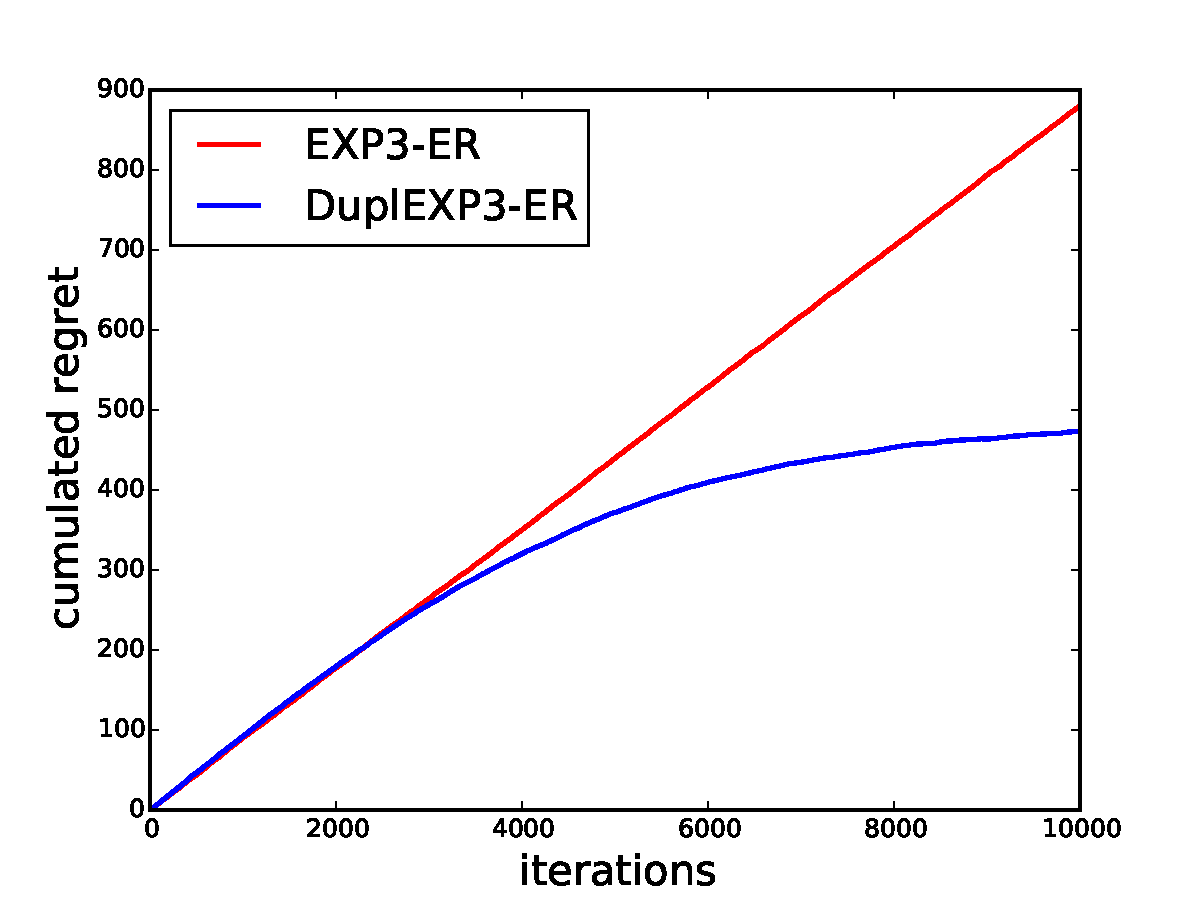
\includegraphics[height=6cm]{figures/50new_dupl_big_r05.pdf}
\label{duplexp3vsexp3ER}
\caption{Comparison of cumulated regret over iterations for EXP3 and DuplExp3 algorithms for and ER graph of 50 nodes with parameter $p=0.5$ (repeated 100 times)}
\end{figure}

\section{BA graphs}
\subsection{Empirical properties of BA graphs}
\paragraph{Independence Number}
Considering the induced hub structure on BA graphs, we conjecture that for the same edge proportion, the mean independence number is higher for BA graphs than for ER graphs. Our conjecture holds true empirically, as shown in Fig~\ref{mean_alpha_ba_er}.

\begin{figure}
 %\includegraphics{figures/mean_alpha_ba_er.eps}
 \label{mean_alpha_ba_er}
 \caption{Average independence number for ER and BA graphs with equal edge proportion}
\end{figure}

\paragraph{Estimated r}
proof of $\E[M_t] \leq \frac{1}{p}$ ??
si pas proof et figure : figure
si rien ... rien


\subsection{Algorithms on BA graphs}
\subsubsection{Asymptotic regime}
As the number of nodes in a BA graph grows, the degree distribution becomes more and more independent of it's initial states and parameter. 
\begin{figure}
 %\includegraphics{figures/dupl_er_ba.eps}
 \label{dupl_er_ba}
 \caption{Average regret for DuplExp3 on BA and ER graphs with the same proportion of edges.}
\end{figure}
\subsubsection{Finite regime}
\paragraph{DuplExp3 on BA Graphs}
To show that the conjecture above indeed lead to an increased regret for \emph{DuplExp3}, we compare regrets of our implementations on ER and BA graphs with the same proportion of edges. Results are shown in Fig~\ref{dupl_er_ba}

\begin{figure}
 %\includegraphics{figures/dupl_er_ba.eps}
 \label{dupl_er_ba}
 \caption{Average regret for DuplExp3 on BA and ER graphs with the same proportion of edges.}
\end{figure}

We tried applying the asymptotic \emph{revelation probabillity} to small ($250$ nodes) BA graphs, which led to the plot in Fig~\ref{dupl_ba_finite_ba}.

\begin{figure}
% \includegraphics{figures/dupl_ba_finite_ba.eps}
 \label{dupl_ba_finite_ba}
 \caption{Average regret for DuplExp3 on BA and ER graphs with the same proportion of edges.}
\end{figure}


\section{Conclusion}
gargl


\end{document}